\chapter{Overview}

This section aims to briefly introduce the Raspberry Pi 4, give a clear overview of the physical testbed and the network topology.


\section{The Raspberry Pi 4 Cluster} \label{pi4cluster}

The Raspberry Pi is a series of small single-board computers developed in the United Kingdom by the Raspberry Pi Foundation to promote teaching of basic computer science in schools and in developing countries. The Raspberry Pi 4 Model B was released in 2019, and is the model used in this cluster.

\begin{table}[H]
    \centering
    \begin{tabular}{ |p{4cm}|p{2cm}|p{4cm}|p{2cm}|p{2cm}|  }
        \hline
        \multicolumn{5}{|c|}{\textbf{Raspberry Pi 4 Model B Specifications}} \\
        \hline
        \textbf{CPU} & \textbf{RAM} & \textbf{NICs} & \textbf{Storage} & \textbf{USB}\\
        \hline
        Broadcom BCM2711 \newline Cortex-A72 (ARMv8) 64-bit SoC \newline 1.5GHz, Quad-core &
        4GB LPDDR4-2400 SDRAM &
        Gigabit Ethernet Controller (part of CPU) \newline Dual IEEE 802.11ac WiFi 5, Bluetooth 5.0 &
        32GB Micro-SD &
        2 USB 3.0 ports \newline 2 USB 2.0 ports\\
        \hline
    \end{tabular}
    \caption{The hardware specifications of Raspberry Pi 4 Model B.}
\end{table}

The cluster consists of eight Raspberry Pi 4 Model B machines, all hooked up to a Zyxel switch. The switch provides interconnectivity, but also powers the machines through \gls{poe}.

\begin{figure}[H]
    \centering
    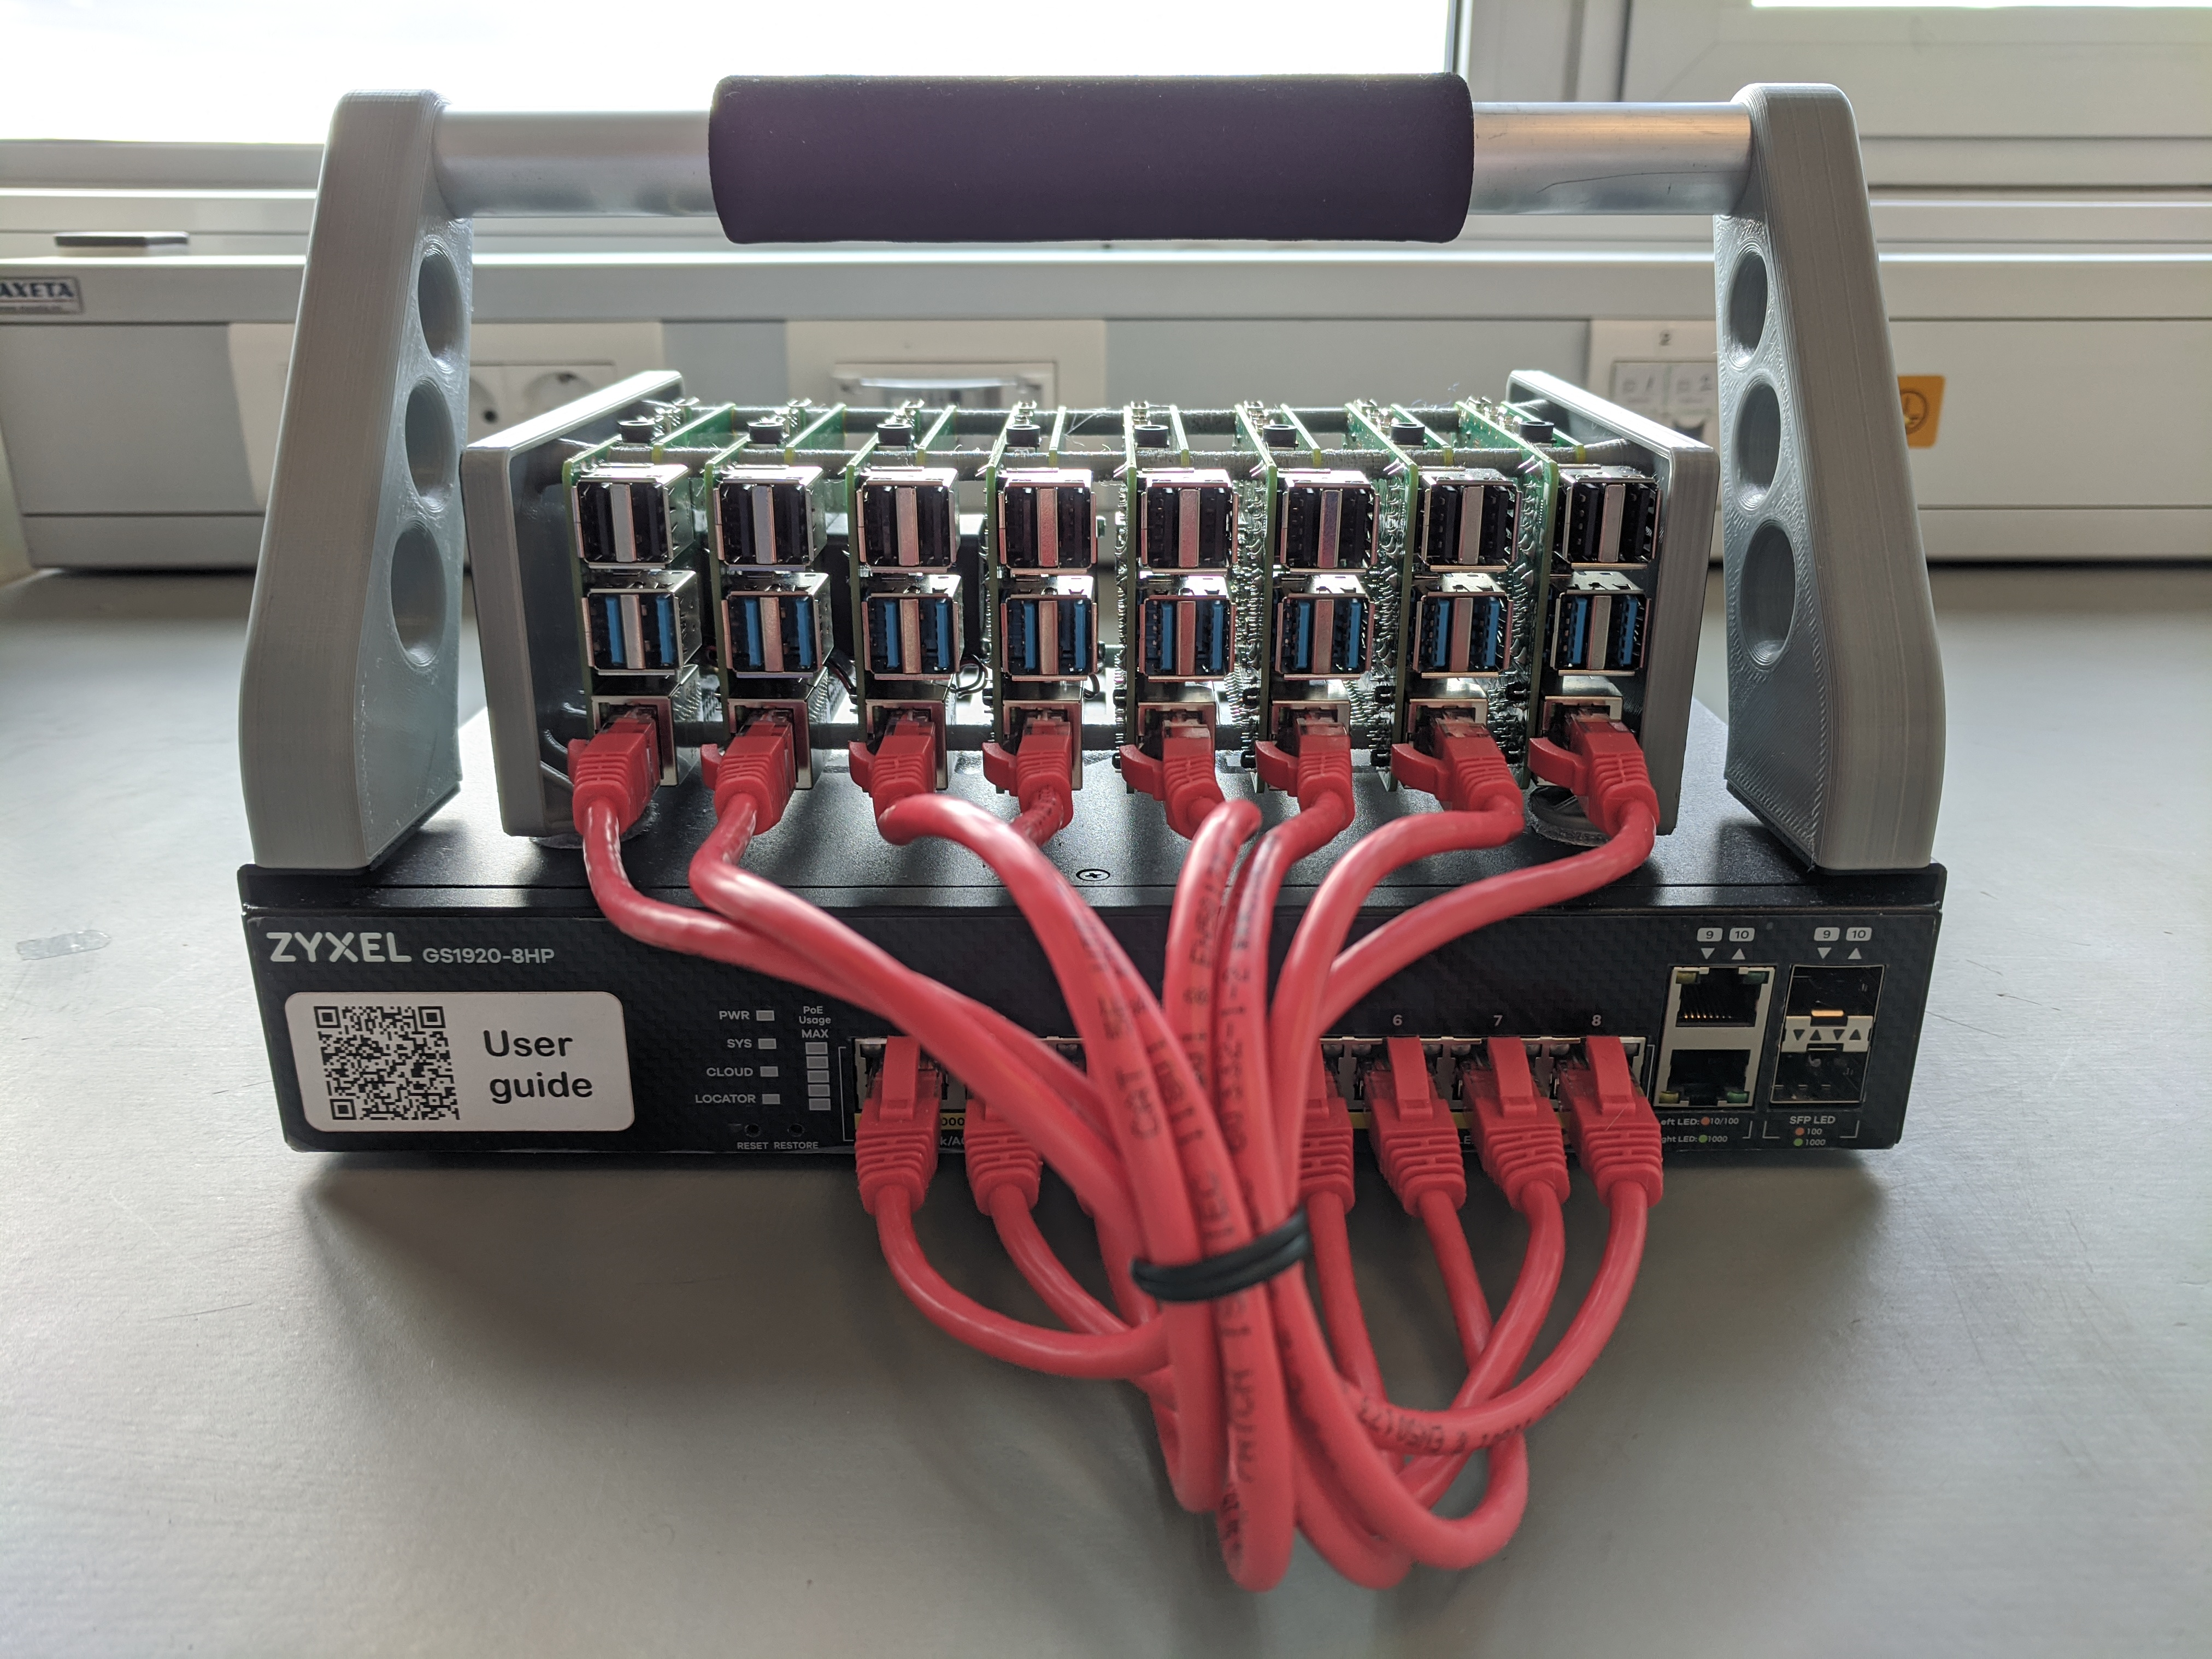
\includegraphics[width=0.6\linewidth]{pi4cluster}
    \captionsetup{width=0.6\linewidth}
    \caption{The Raspberry Pi 4B cluster all hooked to a Zyxel switch.}
    \label{fig:pi4cluster}
\end{figure}

\section{Network Topology} \label{topology}

The testbed consists of two networks; the \textit{controller} network in which all machines are connected directly, and the \textit{experimental} network separated by two subnets with a router in-between.

\begin{figure}[H]
    \centering
    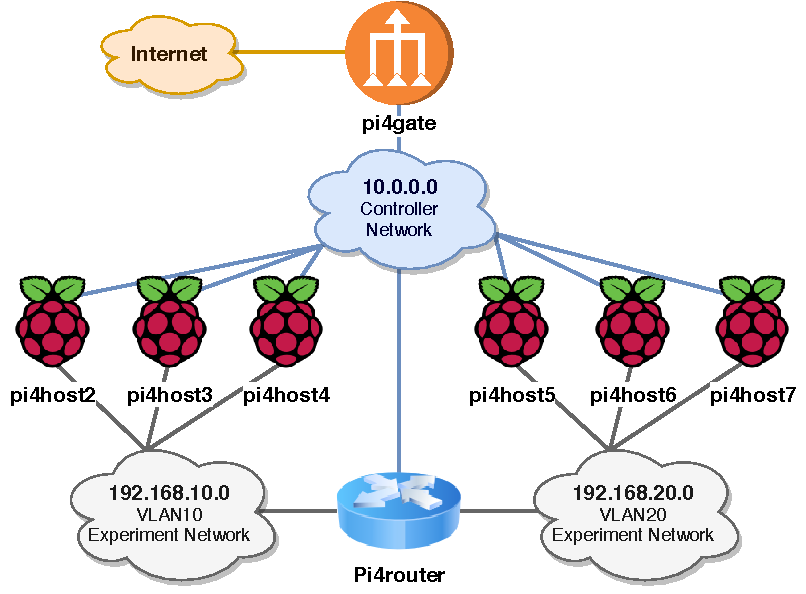
\includegraphics[width=0.8\linewidth]{network_topology}
    \captionsetup{width=0.8\linewidth}
    \caption{The logical network topology for the Raspberry Pi 4B cluster testbed.}
    \label{fig:network_topology}
\end{figure}

Since the entire testbed is connected to a single switch only, both \gls{vlan} and virtual interfaces have been used to achieve the desired network topology. In addition, one USB-to-ethernet adapter was necessary on the router in order to conduct network experimentation with TEACUP. The \gls{vlan} setup on the switch is explained in section \ref{zyxel} while the general network setup for every machine is explained in the remaining sections.

A summary table of the network setup for each machine follows.

\begin{table}[H]
    \centering
    \begin{tabular}{ |p{2cm}|p{6cm}|p{3cm}|  }
        \hline
        \multicolumn{3}{|c|}{\textbf{Summary Network Setup}} \\
        \hline
        \textbf{Hostname} & \textbf{IP address} & \textbf{OS}\\
        \hline
        pi4router & 10.0.0.1 --- eth0 \newline 192.168.10.1 --- eth0:10 (virtual) \newline 192.168.20.1 --- eth1 (USB-to-eth) & Raspbian Buster (Linux)\\
        \hline
        pi4host2 & 10.0.0.2 --- eth0 \newline 192.168.10.2 --- eth0:10 (virtual) & Raspbian Buster (Linux)\\
        \hline
        pi4host3 & 10.0.0.3 --- eth0 \newline 192.168.10.3 --- eth0:10 (virtual) & Raspbian Buster (Linux)\\
        \hline
        pi4host4 & 10.0.0.4 --- eth0 \newline 192.168.10.4 --- eth0:10 (virtual) & Raspbian Buster (Linux)\\
        \hline
        pi4host5 & 10.0.0.5 --- eth0 \newline 192.168.20.5 --- eth0:20 (virtual) & Raspbian Buster (Linux)\\
        \hline
        pi4host6 & 10.0.0.6 --- eth0 \newline 192.168.20.6 --- eth0:20 (virtual) & Raspbian Buster (Linux)\\
        \hline
        pi4host7 & 10.0.0.7 --- eth0 \newline 192.168.20.7 --- eth0:20 (virtual) & Raspbian Buster (Linux)\\
        \hline
        pi4gate & DHCP --- eth0 \newline 10.0.0.254 --- eth0:1 (virtual) & Raspbian Buster (Linux)\\
        \hline
    \end{tabular}
    \caption{The hostnames, IP addresses and OS for each Raspberry Pi 4B machine in the cluster.}
\end{table}

The table above lists the configured Raspberry Pi 4B machines in left to right order as seen from \ref{fig:pi4cluster}. That is, the left most machine is set up as the router, and the right most machine is set up as the gateway.